
\documentclass[xcolor={usenames,dvipsnames},10pt,presentation,aspectratio=169]{beamer}

\usepackage[utf8]{inputenc}
\usepackage[brazilian]{babel}
\usepackage{verbatim}
\usepackage{graphicx}
\usepackage{xspace}
\usepackage{amsthm}
\usepackage{url}
\usepackage{array}
\usepackage{hyperref}
\usepackage{times,mathptmx}
\usepackage{pdfpages}
\usepackage{mdframed}
\usepackage{tikz}
\usepackage{alltt}
%\usepackage[usenames,dvipsnames]{xcolor}
%\usepackage[usenames,dvipsnames]{color}
%\usepackage{color}

\usetikzlibrary{arrows,shapes}

\usetheme{Madrid}
%\usetheme{Boadilla}
%\usetheme{Darmstadt}
%\usetheme{Frankfurt}
%\usetheme{CambridgeUS}
%\usetheme{AnnArbor}
%\usecolortheme{beaver}
%\usecolortheme{seahorse}
%\usecolortheme{seagull}
\usecolortheme[named=BrickRed]{structure}

\setbeamercovered{transparent}

\setbeamertemplate{footline}[frame number]
%\setbeamertemplate{navigation symbols}{}
%\setbeamersize{text margin left=1em,text margin right=1em}

\newcommand{\titulo}{Introdução C++}
\newcommand{\disciplina}{ELC1067 - Laboratório de Programação II}
\newcommand{\nome}{João Vicente Ferreira Lima (UFSM)}

\lecture[1]{\aula}{aula01}
\def\lecturename{\aula}

\newcommand{\Red}[1]{{\color{red}#1}}
\newcommand{\red}[1]{{\color{red}#1}}
\newcommand{\Blue}[1]{{\color{blue}#1}}
\newcommand{\blue}[1]{{\color{blue}#1}}

\newcommand{\PBS}[1]{\let\temp=\\#1\let\\=\temp}
\newcommand{\RRCOL}{\PBS\raggedright\hspace{0pt}}

\newcommand{\p}[1]{\texttt{#1}}
\newenvironment{code}{%
  \begin{alltt}%
  }{%
  \end{alltt}%
}

\makeatletter
%\setbeamertemplate{headline}{}
% {%
%   \leavevmode%
%   \@tempdimb=2.4375ex%
%   \ifnum\beamer@subsectionmax<\beamer@sectionmax%
%     \multiply\@tempdimb by 4%
%   \else%
%     \multiply\@tempdimb by\beamer@subsectionmax%
%   \fi%
%   \ifdim\@tempdimb>0pt%
%     \advance\@tempdimb by 1.125ex%
%     \begin{beamercolorbox}[wd=.5\paperwidth,ht=\@tempdimb]{section in head/foot}%
%       \vbox to\@tempdimb{\vfil\insertsectionnavigation{.5\paperwidth}\vfil}%
%     \end{beamercolorbox}%
%     \begin{beamercolorbox}[wd=.45\paperwidth,ht=\@tempdimb]{subsection in head/foot}%
%       \vbox
%       to\@tempdimb{\vfil\insertsubsectionnavigation{.45\paperwidth}\vfil}%
%     \end{beamercolorbox}%
%     \begin{beamercolorbox}[wd=.05\paperwidth,ht=\@tempdimb]{subsection in head/foot}%
%       \vbox
%       to\@tempdimb{\vfil\hfil\insertframenumber\vfil\vfil}%
%     \end{beamercolorbox}%
%   \fi%
% }

\def\dohead{\beamer@headcounter=4\relax\beamer@headcounter=1\loop\ifnum\beamer@headcounter<\beamer@totalheads%
  \advance\beamer@headcounter by1\relax%
  \csname @@head\the\beamer@headcounter\endcsname\repeat}

\makeatother

\title[\titulo]{\titulo}

\subtitle{\disciplina}

\author[João V. F. Lima]{\nome}

%\institute[UFSM]{Departamento de Linguagens e Sistemas de Computação \\ Universidade Federal de Santa Maria \\ \url{jvlima@inf.ufsm.br} \\ \url{http://www.inf.ufsm.br/~jvlima}}
\institute[UFSM]{Universidade Federal de Santa Maria \\ \url{jvlima@inf.ufsm.br} \\ \url{http://www.inf.ufsm.br/~jvlima}}
\date{2023/1}

\graphicspath{{.}{figs/}}

\logo{ 
\includegraphics[height=1.5cm,width=1.5cm,keepaspectratio]{logo_inf}    
        
\includegraphics[height=1.5cm,width=1.5cm,keepaspectratio]{logo_ufsm} }

%\titlegraphic{
%	
\includegraphics[width=2cm]{logo_ufsm}
%  \hspace{1cm}
%	
\includegraphics[width=2cm]{logo_inf}
%}

\newtheorem{mydef}{Definição}[section]
%\newtheorem{myteo}{Teorema}[section]
%------------------------------------------------------------------------------
%\newcommand{\xkaapi}{XKaapi\xspace}
%------------------------------------------------------------------------------
% Typesetting Listings
\usepackage{listings}
\lstset{
  language=C++,
  %basicstyle=\scriptsize\ttfamily,
  %basicstyle=\normalsize\ttfamily,
  basicstyle=\small\ttfamily,
  %basicstyle=\footnotesize\ttfamily,
  aboveskip=0pt,
  belowskip=0pt,
  mathescape=false,
  columns=flexible,
  numbers=none,
%  numbers=left,
%  showtabs=true,
%  showspaces=true,
  breaklines=true
}
%------------------------------------------------------------------------------
\lstset{commentstyle=\color{blue}}
%\lstset{stringstyle=\ttfamily}
%\lstset{ classoffset=1, 
%            morekeywords={kaapi,omp,task,data,alloca, declare, reduction, identity, parallel,sync,taskwait,cilk,spawn,tbb,css,cilk\_spawn,cilk\_sync,cilk\_for,offload},
%            keywordstyle=\color{Red}\bfseries
%           }
%\lstset{ classoffset=2, 
%            morekeywords={value,read,write,readwrite,reduction,untied,firstprivate,TaskBodyCPU,TaskBodyGPU,ka,Signature,RW,CW,range2d\_r,range2d\_rw,range2d,Spawn,Fork,Shared\_w,Shared\_r,Shared,a1,target,device,copyin,copyout,input,implements,copy\_deps,RPWP,range2d\_rpwp,rangeindex,Memory,Register,SetStaticSched,Sync,Unregister,Community,System,join\_community,SpawnMain,leave,initialize,terminate,logfile,array,SetArch,ArchHost,ArchCUDA,W,R,gpuStream,pointer\_w,pointer\_r,pointer\_cw,pointer},
%            keywordstyle=\color{Blue}\bfseries
%           }
%\lstset{ classoffset=3, 
%            morekeywords={storage,ld},
%            keywordstyle=\bfseries
%           }
%\lstset{ classoffset=4, 
%            morekeywords={in,out,inout,cout,concurrent},
%            keywordstyle=\color{Red}\bfseries
%           }
%           
\lstset{classoffset=0, showstringspaces=false}
%------------------------------------------------------------------------------
\mdfsetup{
  backgroundcolor=gray!10,
%  roundcorner=10pt,
}
%------------------------------------------------------------------------------
\newcommand{\restorefootline}{\setbeamertemplate{navigation symbols}{}}
%\newcommand{\setfootline}[1]{\setbeamertemplate{navigation symbols}{\textcolor{black}{\textbf{#1}}}}
\newcommand{\includeslides}[4]{%
  %\setfootline{#1}%
  {
    \setbeamercolor{background canvas}{bg=}
    \includepdf[pages={#2},%
    pagecommand={},
%    pagecommand={\begin{frame}[default]{}\end{frame}},
    #4,%
    turn=false,noautoscale=false,column=false,columnstrict=false,openright=false,frame=false]{#3}%
  }
  %\restorefootline%
}
%------------------------------------------------------------------------------
\begin{document}

\begin{frame}
%  \titlepage
  \maketitle
%  \mode<presentation>
%  {
%    \begin{columns}
%      \begin{column}{0.5\textwidth}
%      \raggedleft
%	
\includegraphics[width=2cm]{logo_ufsm}
%      \end{column}
%      \begin{column}{0.5\textwidth}
%	
\includegraphics[width=2cm]{logo_inf}
%      \end{column}
%    \end{columns}
%  }
\end{frame}

\begin{frame}
    \frametitle{Outline}
    \tableofcontents[hideallsubsections]
%    \tableofcontents
\end{frame}

\AtBeginSection{
  \begin{frame}
    \frametitle{Outline}
    \tableofcontents[currentsection,hideothersubsections]
  \end{frame}
}

%%%%%%%%%%%%%%%%%%%%%%%%%%%%%%%%%%%%%%%%%%%%%%%%%%%%%%%%%%%%%%%%%%%%%%%%%%%%%%
\section{Introdução}
%%%%%%%%%%%%%%%%%%%%%%%%%%%%%%%%%%%%%%%%%%%%%%%%%%%%%%%%%%%%%%%%%%%%%%%%%%%%%%%
%------------------------------------------------------------------------------
\begin{frame}
  \frametitle{Unix history}
UNIX was written in assembly by Ken Thompson at Bell Labs (AT\&T) in
1969 for a Digital PDP-7 minicomputer. It took several ideias from
MULTICS such as:
\begin{columns}\begin{column}{0.7\textwidth}
  \begin{itemize}
    \item tree-structured file system.
    \item separate program for interpreting commands (shell).
    \item notion of files as unstructured streams of bytes.
  \end{itemize}
\end{column}\begin{column}{0.3\textwidth}
\begin{center}
  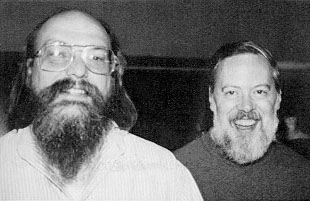
\includegraphics[width=0.7\textwidth]{ken_denis}
\end{center}
\end{column}\end{columns}

Denis Ritchie designed and implemented C language between 1969-1973
at Bell Labs. By 1973, UNIX was almost totally written in C.
\begin{block}{C for system programming}
In the 70s, widely used languages were designed to other purposes:
  \begin{itemize}
    \item FORTRAN for mathematical tasks
    \item COBOL for commercial systems 
  \end{itemize}
\end{block}
\end{frame}
%------------------------------------------------------------------------------
\begin{frame}
  \frametitle{Visão de computador}
    \begin{columns}
      \begin{column}{0.4\textwidth}
      \raggedleft
        O \textbf{sistema operacional} e as \textbf{linguagens de programação} criam uma interface ao computador
     \end{column}
      \begin{column}{0.6\textwidth}
  \begin{center}
	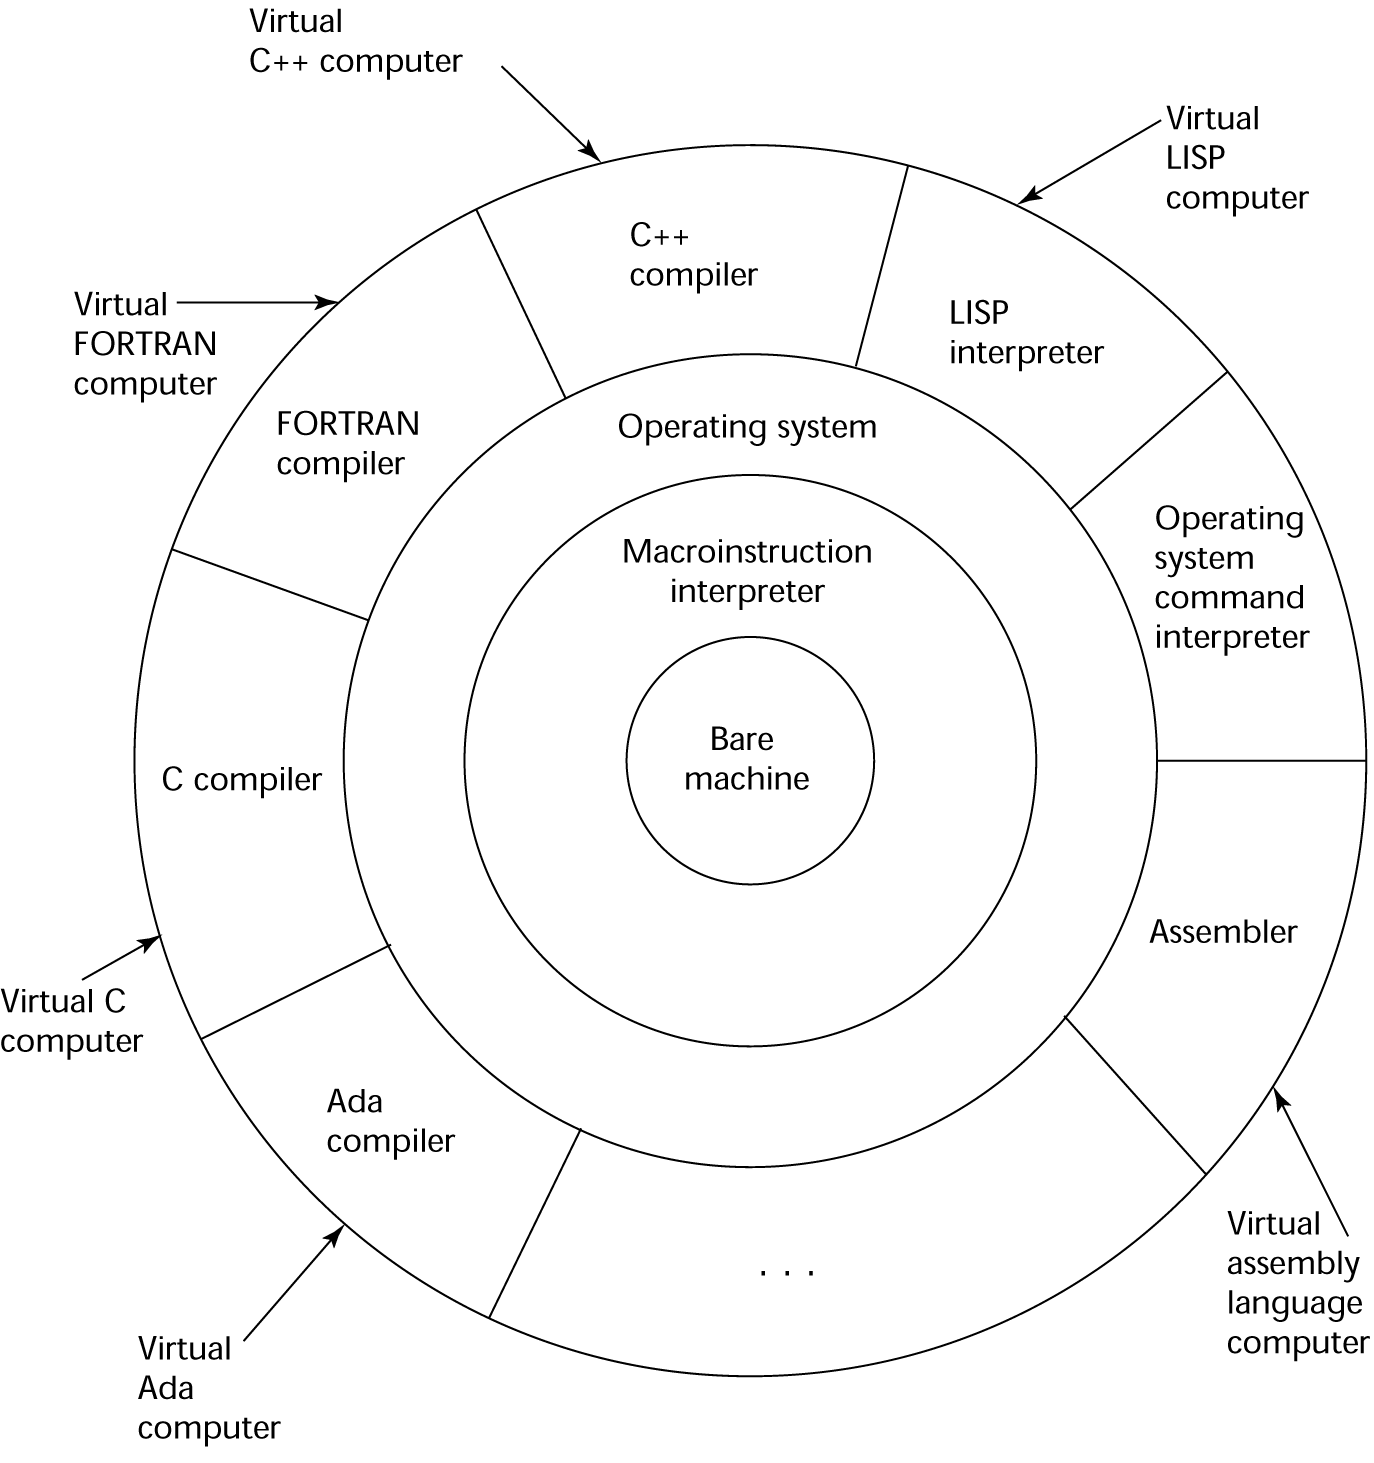
\includegraphics[width=0.8\textwidth]{vm.png}
  \end{center}
      \end{column}
    \end{columns}
\end{frame}
%------------------------------------------------------------------------------
\begin{frame}
  \frametitle{História do C++}
    \begin{columns}
      \begin{column}{0.7\textwidth}
        \begin{itemize}
          \item Criado em 1979 como \emph{C with Classes} por Bjarne Stroustrup
          \item C++ é compatível com C
          \item Abstrações sem comprometer o desempenho 
          \item 1985: primeira edição do livro \emph{The C++ Programming Language}
          \item 1994: STL (\emph{Standard Template Library}) por Alexander Stepanov
          \item 1998: ISO C++ standard.
        \end{itemize}
     \end{column}
      \begin{column}{0.3\textwidth}
  \begin{center}
	
\includegraphics[width=0.8\textwidth]{4thEnglish.jpeg}
  \end{center}
      \end{column}
    \end{columns}
\end{frame}
%------------------------------------------------------------------------------
\begin{frame}
  \frametitle{História do C++}
  \begin{center}
	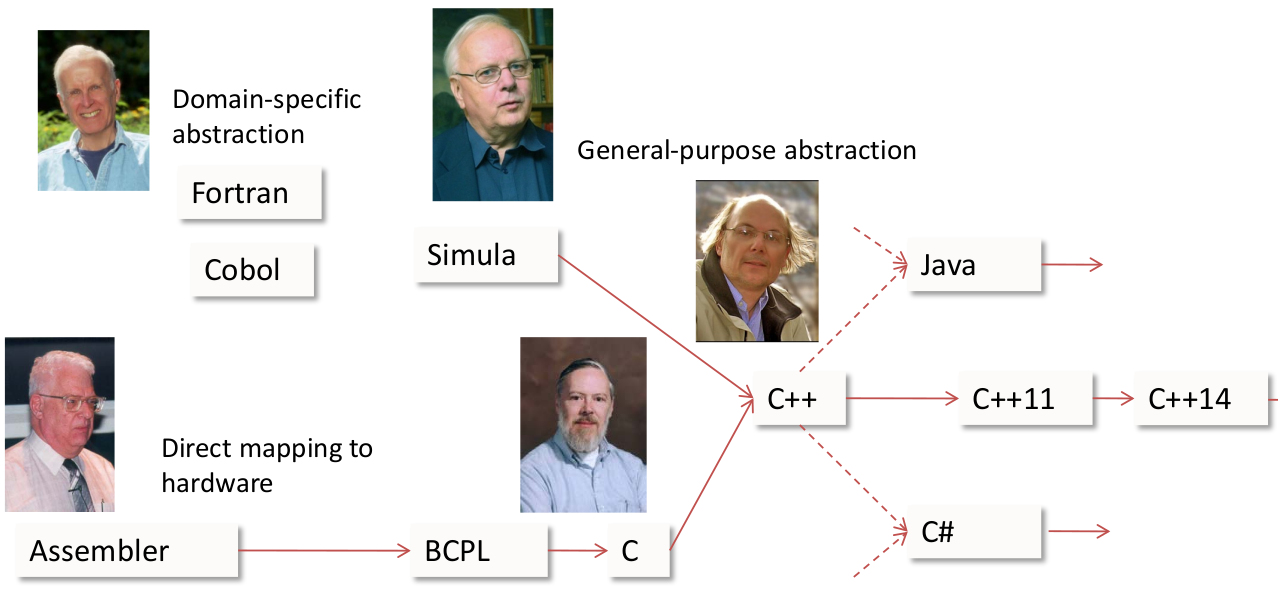
\includegraphics[width=0.8\textwidth]{roots_cpp.png}
  \end{center}
  {\footnotesize Bjarne Stroustrup, \emph{The Evolution of C++: Past, Present, and Future}, CppCon 2016 \\ \url{https://youtu.be/\_wzc7a3McOs}}
\end{frame}
%------------------------------------------------------------------------------
\begin{frame}
  \frametitle{História do C++}
  \begin{center}
	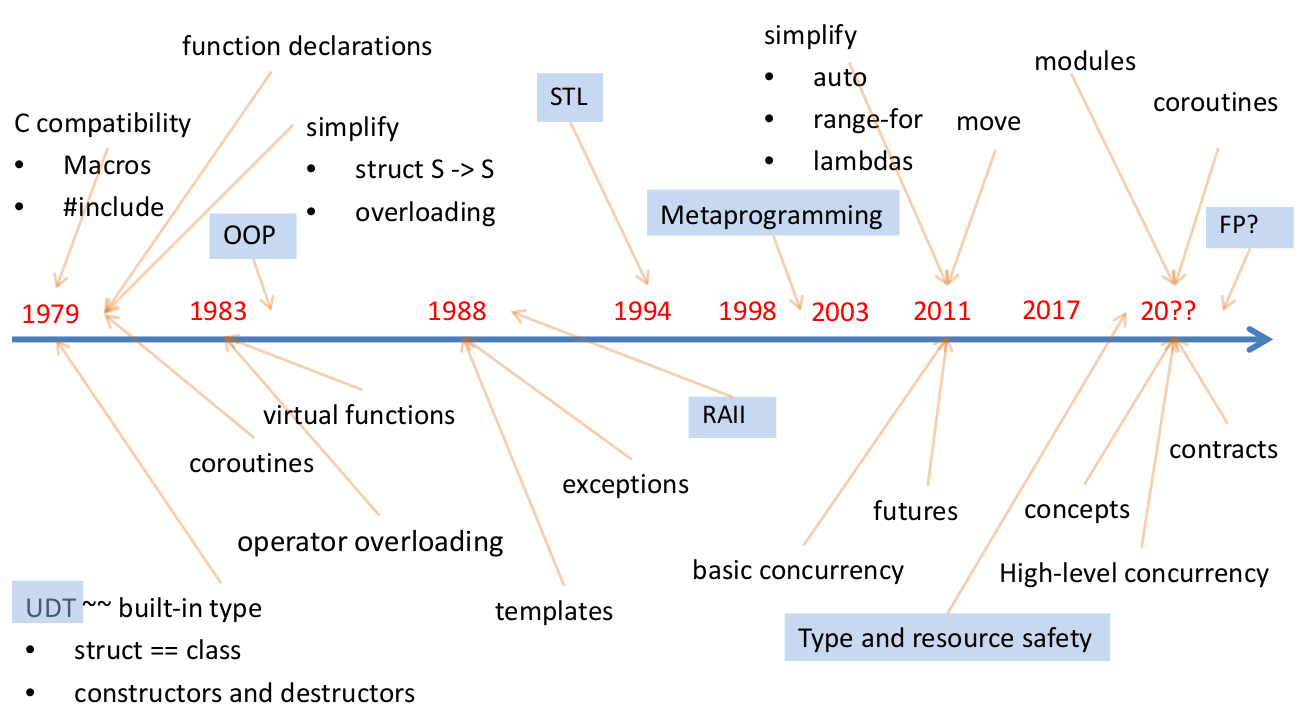
\includegraphics[width=0.8\textwidth]{cpptimeline.png}
  \end{center}
  {\footnotesize Bjarne Stroustrup, \emph{The Evolution of C++: Past, Present, and Future}, CppCon 2016 \\ \url{https://youtu.be/\_wzc7a3McOs}}
\end{frame}
%------------------------------------------------------------------------------
\begin{frame}
  \frametitle{História do C++}
  \begin{center}
	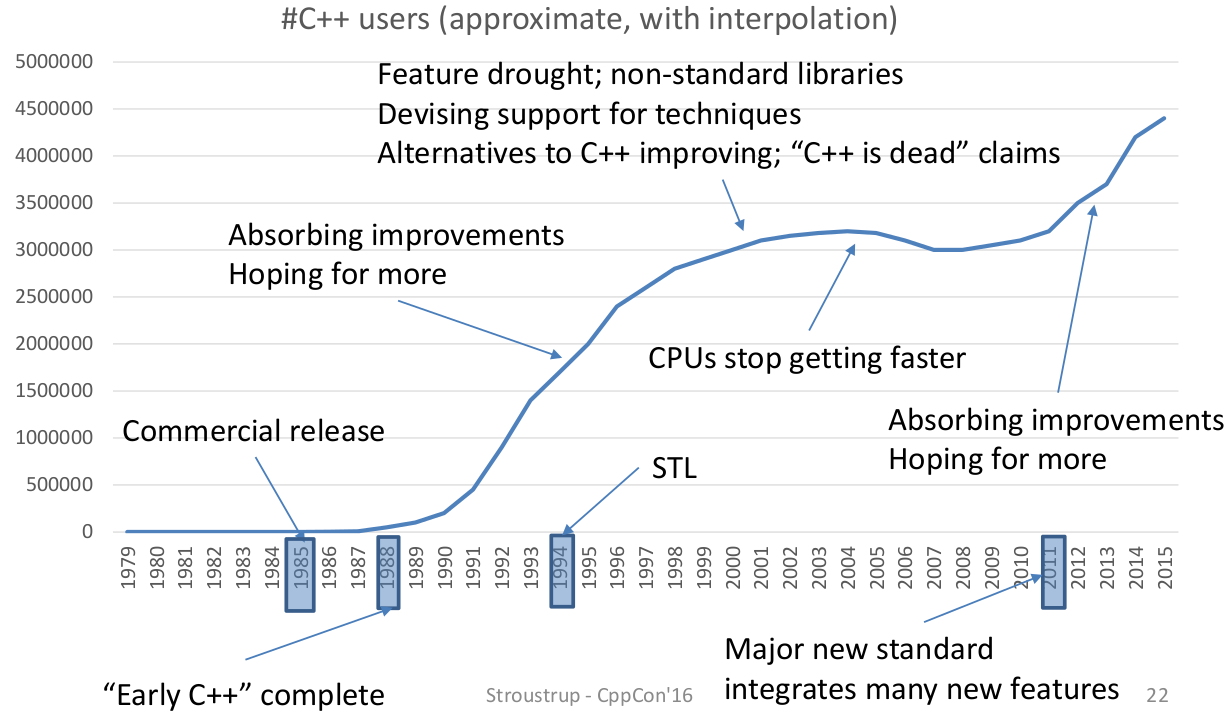
\includegraphics[width=0.8\textwidth]{cppsuccess.png}
  \end{center}
  {\footnotesize Bjarne Stroustrup, \emph{The Evolution of C++: Past, Present, and Future}, CppCon 2016 \\ \url{https://youtu.be/\_wzc7a3McOs}}
\end{frame}
%------------------------------------------------------------------------------
% TODO: excessao, etc
%\begin{frame}
%  \frametitle{Entrada e saída}
%  \begin{itemize}
%  \item 
%  \end{itemize}
%\end{frame}
%------------------------------------------------------------------------------
\begin{frame}
  \frametitle{Stack Overflow}
  \vspace{-2mm}
  \begin{center}
	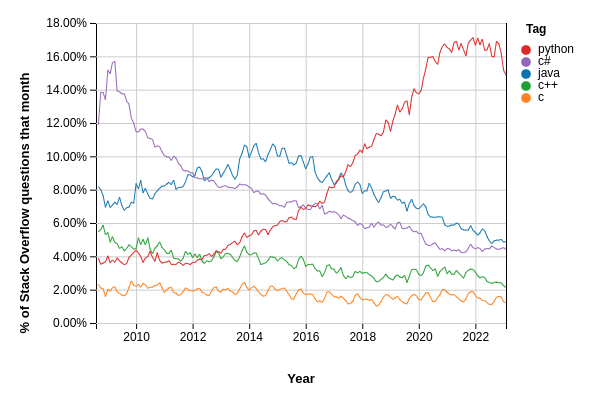
\includegraphics[width=0.7\textwidth]{stackoverflow.png}
  \end{center}
  \vspace{-7mm}
  {\footnotesize Fonte: \url{https://insights.stackoverflow.com/}}
\end{frame}
%------------------------------------------------------------------------------
\begin{frame}
  \frametitle{Compilação de programas}
  \begin{center}
  \begin{tikzpicture}[block/.style={
      draw,
      shape=rectangle,
      align=center,
      node distance=3cm,
      black,
      very thick
    }
    ]
    %\draw (0,0) node [draw, black, very thick] {Código};
    %\draw (0,0) node {A} -> (1,0) node {B};
    %\draw[->] 0,
    \node[block] (A) at (0,0) {\textsc{Código C++}};
    \node[block,right of=A] (B) {\textsc{Compilador}};
    \node[block,right of=B] (F) {\textsc{Código objeto}};
    \node[block,right of=F] (C) {\textsc{Ligador}};
    \node[block,right of=C] (D) {\textsc{Executável}};
    \node[block,below of=C] (E) {\textsc{Bibliotecas (DLLs, so)}};
    \draw[->,very thick] (A) -- (B);
    \draw[->,very thick] (B) -- (F);
    \draw[->,very thick] (F) -- (C);
    \draw[->,very thick] (C) -- (D);
    \draw[->,very thick] (E) -- (C);
  \end{tikzpicture}
  \end{center}
\end{frame}
%------------------------------------------------------------------------------
%\begin{frame}
%  \frametitle{Entrada e saída}
%  \begin{itemize}
%  \item 
%  \end{itemize}
%\end{frame}
%------------------------------------------------------------------------------
%------------------------------------------------------------------------------
\begin{frame}[fragile]
  \frametitle{Olá mundo}
  \vspace{-2mm}
    \begin{columns}
      \begin{column}{0.5\textwidth}
          \begin{itemize}
          \item \textbf{iostream} para entrada e saída básica.
          \item \textbf{std::string} é uma estrutura (``classe'') C++ para string.
          \item \textbf{std::cout} é a saída padrão.
          \item \textbf{std::endl} é uma nova linha 
            \begin{itemize}
              \item UNIX/Linux - \texttt{\char`\\n}
              \item Windows - \texttt{\char`\\r\char`\\n}
            \end{itemize}
          \end{itemize}
     \end{column}
      \begin{column}{0.5\textwidth}
%      \begin{center}
  \begin{block}{ola.cpp}
\begin{lstlisting}
#include <iostream>

int main(void)
{
    std::string mensagem{"Ola mundo!"}
    // isso eh um comentario
    std::cout << "Saida: " << mensagem << std::endl;
    return 0;
}
\end{lstlisting}
\end{block}
%      \end{center}
      \end{column}
    \end{columns}
%
%
\end{frame}
%------------------------------------------------------------------------------
\begin{frame}[fragile]
  \frametitle{Compilador}
\begin{exampleblock}{Instalação do GCC em sistemas Debian/Ubuntu}
\begin{lstlisting}
$ apt install gcc g++
\end{lstlisting}
\end{exampleblock}
%
\begin{exampleblock}{Instalar ferramentas essenciais}
\begin{lstlisting}
$ apt install make valgrind gdb cppcheck 
\end{lstlisting}
\end{exampleblock}
%
\begin{alertblock}{Dica}
Semelhante ao C, pode-se usar o \textbf{GCC} (\texttt{g++}) e \textbf{Clang}
(\texttt{clang++}).
Clang mostra erros de compilação de forma mais amigável, além de ser mais 
eficiente que o GCC.
\end{alertblock}
\end{frame}
%------------------------------------------------------------------------------
\begin{frame}[fragile]
  \frametitle{Compilação}
\begin{exampleblock}{Linha de comando}
\begin{lstlisting}
$ g++ -std=c++11 -O2 -Wall -g  -o ola ola.cpp
$ ./ola
\end{lstlisting}
\end{exampleblock}
%
\begin{exampleblock}{Linha de comando (alternativa)}
\begin{lstlisting}
$ g++ -std=c++11 -O2 -Wall -g ola.cpp
$ ./a.out
\end{lstlisting}
\end{exampleblock}
\end{frame}
%------------------------------------------------------------------------------
\begin{frame}[fragile]
  \frametitle{Linha de comando}
  \begin{block}{params.cpp}
\begin{lstlisting}
#include <iostream>

// argc eh o numero de parametros passados
// argv eh um vetor de strings com os valores
int main(int argc, char **argv)
{
    for(auto i= 0; i < argc; i++){
        std::cout << "Param " << i
            << " valor -> " << argv[i] << std::endl;
    }
    return 0;
}
\end{lstlisting}
  \end{block}
\end{frame}
%------------------------------------------------------------------------------
%%%%%%%%%%%%%%%%%%%%%%%%%%%%%%%%%%%%%%%%%%%%%%%%%%%%%%%%%%%%%%%%%%%%%%%%%%%%%%%
\section{Variáveis}
%%%%%%%%%%%%%%%%%%%%%%%%%%%%%%%%%%%%%%%%%%%%%%%%%%%%%%%%%%%%%%%%%%%%%%%%%%%%%%%
%------------------------------------------------------------------------------
\begin{frame}[fragile]
  \frametitle{\texttt{auto}}
Pode-se usar \textbf{auto} quando o tipo é deduzido pelo compilador.
  \begin{block}{Exemplo}
\begin{lstlisting}
auto x = 1;          // inteiro
auto y = 2.0;        // double
auto teste = true;   // booleano

// i abaixo eh um inteiro
for(auto i= 0; i < 10; i++)
    std::cout << "Valor: " << i << std::endl;
\end{lstlisting}
  \end{block}
\end{frame}
%------------------------------------------------------------------------------
\begin{frame}[fragile]
  \frametitle{Inicialização padrão}
É uma forma de padronizar a inicialização de variáveis em C++ usando \verb+{}+.
  \begin{block}{Exemplos}
\begin{lstlisting}
double x {1.0};                 // declara um double
int    a[] {1, 2, 3, 4};        // vetor com 4 elementos sem = 
int    b[] = {1, 2, 3, 4};      // mesma coisa
std::string nome {"Meu nome"} ; // uma string
\end{lstlisting}
  \end{block}
  %
\begin{alertblock}{Atenção}
Não funciona com \textbf{auto}.
\begin{lstlisting}

auto x {1.0}; // double ou float ?
\end{lstlisting}
\end{alertblock}
\end{frame}
%------------------------------------------------------------------------------
\begin{frame}[fragile]
  \frametitle{Casting (conversão)}
C++ apresenta quatro tipos de conversão:
\begin{itemize}
\item \textbf{static\_cast} - tipos relacionados: \texttt{int} para \texttt{char},
ou \texttt{double*} para \texttt{int*}.
\item \textbf{reinterpret\_cast} - tipos não relacionados (inteiro para ponteiro, etc).
\item \textbf{const\_cast} - \texttt{const} ou \texttt{volatile}.
\item \textbf{dynamic\_cast} (\emph{não usado aqui}).
\end{itemize}
  \begin{block}{Exemplo}
\begin{lstlisting}
int num = 97;                        // inteiro
char letra = static_cast<char>(num); // agora letra A

char *dados = new char[100];          // 100 chars alocados
int* vetor = reinterpret_cast<int*>(dados); // mudei agora para int
\end{lstlisting}
  \end{block}
\end{frame}
%------------------------------------------------------------------------------
\begin{frame}[fragile]
  \frametitle{Passagem por referência}
Passagem por referência possibilita passar variáveis por 
\textbf{referência} (\verb+&+) ao invés de valor ou ponteiro.
  \begin{block}{Exemplo}
\begin{lstlisting}
void f(int val, int& ref)
{
    val++;   // incrementa a copia local de val
    ref++;   // incrementa realmente a variavel
}
\end{lstlisting}
  \end{block}
%
\end{frame}
%------------------------------------------------------------------------------
\begin{frame}[fragile]
  \frametitle{Passagem por referência}
\begin{alertblock}{Importante}
Evite usar passagem por referência porque deixa o programa
mais difícil de entender.
Use apenas quando queremos evitar uma cópia e não vamos alterar a variável (\verb+const+), 
como por exemplo um vetor ou uma string:
\begin{lstlisting}

void imprimir(const std::string& texto) 
{
    std::cout << texto << std::endl; // nao altera variavel
}
\end{lstlisting}
\end{alertblock}
\end{frame}
%------------------------------------------------------------------------------
\begin{frame}[fragile]
  \frametitle{Estrutura de dados}
  \begin{block}{struct Ponto}
\begin{lstlisting}
struct Ponto {
    float x;  // variaveis
    float y;

    // zera o ponto 
    void zera(void) {
        x = 0.0f;
        y = 0.0f;
    }
    // distancia deste ponto (x, y) ate p1
    float distancia(Ponto& p1) const {
        return std::sqrt( std::pow((x-p1.x), 2) + std::pow((y-p1.y), 2) );
    }
};
\end{lstlisting}
  \end{block}
\end{frame}
%------------------------------------------------------------------------------
\begin{frame}[fragile]
  \frametitle{Estrutura de dados}
  \begin{block}{struct Ponto}
\begin{lstlisting}
int main(void)
{
    Ponto p1 {1.0, 1.0};
    Ponto p2;
    p2.zera();
    p2.x = 19.0;
    p2.y = 20.0;

    auto distancia = p1.distancia(p2);
    std::cout << "Distancia: " << distancia << std::endl;
}
\end{lstlisting}
  \end{block}
\end{frame}
%------------------------------------------------------------------------------
%%%%%%%%%%%%%%%%%%%%%%%%%%%%%%%%%%%%%%%%%%%%%%%%%%%%%%%%%%%%%%%%%%%%%%%%%%%%%%%
\section{Containers STL}
%%%%%%%%%%%%%%%%%%%%%%%%%%%%%%%%%%%%%%%%%%%%%%%%%%%%%%%%%%%%%%%%%%%%%%%%%%%%%%%
%------------------------------------------------------------------------------
%------------------------------------------------------------------------------
\begin{frame}[fragile]
  \frametitle{Containers STL}
  \vspace{-2mm}
    \begin{columns}
      \begin{column}{0.5\textwidth}
        A C++ STL (\emph{Standard Template Library}) consiste em iteradores,
        containers (ou TADs), algoritmos, e funções parte da bibliteca padrão
        do C++.
     \end{column}
      \begin{column}{0.5\textwidth}
%      \begin{center}
  \begin{block}{Vetores C++}
\begin{lstlisting}
std::vector<int> v1 = {1, 2, 3, 4};
std::vector<char> v2;

// insere no fim
v1.push_back(5);

// insere no comeco
v1.push_front(0);

// imprime
std::cout << v1[3] << std::endl;

// insere um caractere
v2.push_back('a');
\end{lstlisting}
\end{block}
      \end{column}
    \end{columns}
\end{frame}
%------------------------------------------------------------------------------
%------------------------------------------------------------------------------
\begin{frame}[fragile]
  \frametitle{Containers STL}
  \vspace{-2mm}
    \begin{columns}
      \begin{column}{0.5\textwidth}
        Iteradores são ``ponteiros'' ou ``cursores'' genéricos aos dados dentro de um container.

        Os containers possuem os métodos:
        \begin{itemize}
           \item \texttt{begin()} para começo.
           \item \texttt{end()} para o fim (ou além dele). 
           \item \texttt{last()} para o último elemento.
          \item \texttt{size()} número de elementos.
          \item \texttt{capacity()} capacidade total em memória.
          \item \texttt{clear()} ``limpa'' o container.
        \end{itemize}
        O iterador tem o operador \texttt{*} para acessar o elemento apontado.
     \end{column}
      \begin{column}{0.5\textwidth}
\begin{block}{Vetores C++}
\begin{lstlisting}
std::vector<int> v1 = {1, 2, 3, 4};

for(auto it= v1.begin(); it != v1.end(); it++)
  std::cout << *it;

std::vector<int>::iterator it;
for(it= v1.begin(); it != v1.end(); it++)
  std::cout << *it;
\end{lstlisting}
\end{block}
      \begin{center}
      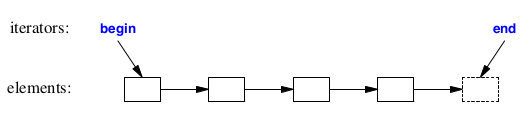
\includegraphics[width=\textwidth]{iterator.png}
      \end{center}
      \end{column}
    \end{columns}
  \onslide<2->
  \begin{center}
  \alert{\large \textbf{Tem como alterar os valores?}}
  \end{center}
\end{frame}
%------------------------------------------------------------------------------
\begin{frame}[fragile]
  \frametitle{Containers STL}
  \vspace{-2mm}
    \begin{columns}
      \begin{column}{0.5\textwidth}
        Iteradores são ``ponteiros'' ou ``cursores'' genéricos aos dados dentro de um container.

        Os containers possuem os métodos:
        \begin{itemize}
           \item \texttt{begin()} para começo.
           \item \texttt{end()} para o fim (ou além dele). 
           \item \texttt{last()} para o último elemento.
          \item \texttt{size()} número de elementos.
          \item \texttt{capacity()} capacidade total em memória.
          \item \texttt{clear()} ``limpa'' o container.
        \end{itemize}
        O iterador tem o operador \texttt{*} para acessar o elemento apontado.
     \end{column}
      \begin{column}{0.5\textwidth}
\begin{block}{Vetores C++}
\begin{lstlisting}
std::vector<int> v1 = {1, 2, 3, 4};

for(auto it= v1.begin(); it != v1.end(); it++)
  *it = *it + 1;
\end{lstlisting}
\end{block}
      \end{column}
    \end{columns}
\end{frame}
%------------------------------------------------------------------------------
%%%%%%%%%%%%%%%%%%%%%%%%%%%%%%%%%%%%%%%%%%%%%%%%%%%%%%%%%%%%%%%%%%%%%%%%%%%%%%%
\section{Entrada e saída}
%%%%%%%%%%%%%%%%%%%%%%%%%%%%%%%%%%%%%%%%%%%%%%%%%%%%%%%%%%%%%%%%%%%%%%%%%%%%%%%
%------------------------------------------------------------------------------
\begin{frame}[fragile]
  \frametitle{Entrada e saída}
As operações são efetuadas por \textbf{streaming} ou fluxo onde dados:
\begin{itemize}
\item \textbf{std::ifstream} para leitura (operador \verb+>>+).
\item \textbf{std::ofstream} para escrita (operador \verb+<<+).
\end{itemize}
  \begin{block}{Exemplo}
\begin{lstlisting}
#include <iostream>
#include <fstream>

int main(void)
{
    int n1, n2;
    std::ifstream entrada {"entrada.txt"};
    std::ofstream saida {"saida.txt"};
    entrada >> n1 >> n2;
    saida << n1 << " " << n2 << std::endl;
    return 0;
}
\end{lstlisting}
  \end{block}
\end{frame}
%------------------------------------------------------------------------------
\begin{frame}[fragile]
  \frametitle{Entrada e saída}
  \begin{block}{EOF - \emph{end-of-file}}
\begin{lstlisting}
#include <iostream>
#include <fstream>
int main(void) {
    int n;
    std::ifstream entrada {"numeros.txt"};
    std::ofstream saida {"saida.txt"};
    if(entrada.is_open() == false)
        throw std::runtime_error{"ERRO arquivo!"};

    while(entrada.eof() == false){
        entrada >> n;
        saida << n << std::endl;
    }
    entrada.close();
    saida.close();
    return 0;
}
\end{lstlisting}
  \end{block}
\end{frame}
%------------------------------------------------------------------------------
\begin{frame}[fragile]
  \frametitle{Entrada e saída}
  \begin{block}{Ler linha em C++ (continua)}
\begin{lstlisting}
#include <iostream>
#include <fstream>
#include <vector>

struct Aluno {
    int matricula;
    std::string nome;
};
\end{lstlisting}
  \end{block}
\end{frame}
%------------------------------------------------------------------------------
\begin{frame}[fragile]
  \frametitle{Entrada e saída}
  \begin{block}{Ler linha em C++}
\begin{lstlisting}
int main(void)
{
    int matricula;
    std::string nome;
    std::vector<Aluno> alunos;             // vetor de alunos
    std::ifstream entrada {"alunos.txt"};
    while( entrada >> matricula ) { // le matricula 
        std::getline(entrada, nome); // le resto da linha
        alunos.push_back( Aluno{matricula, nome} );
    }

    for(Aluno& v: alunos)
        std::cout << v.matricula << " -> " << v.nome << std::endl;
    return 0;
}
\end{lstlisting}
  \end{block}
\end{frame}
%------------------------------------------------------------------------------
%%%%%%%%%%%%%%%%%%%%%%%%%%%%%%%%%%%%%%%%%%%%%%%%%%%%%%%%%%%%%%%%%%%%%%%%%%%%%%%
\section{Escopos}
%%%%%%%%%%%%%%%%%%%%%%%%%%%%%%%%%%%%%%%%%%%%%%%%%%%%%%%%%%%%%%%%%%%%%%%%%%%%%%%
%------------------------------------------------------------------------------
\begin{frame}[fragile]
  \frametitle{Namespaces}
  \vspace{-2mm}
    \begin{columns}
      \begin{column}{0.4\textwidth}
Namespaces em C++ são \textbf{escopos nomeados}  e aumenta a modularidade do código.
A \verb+std+ é o namespace padrão do C++.
     \end{column}
      \begin{column}{0.6\textwidth}
%      \begin{center}
  \begin{block}{}
\begin{lstlisting}
#include <iostream>

int main(void)
{
  std::string mensagem{"Ola mundo!"}
  std::cout << << mensagem << std::endl;
  return 0;
}
\end{lstlisting}
\end{block}
%      \end{center}
      \end{column}
    \end{columns}
%
\end{frame}
%------------------------------------------------------------------------------
%------------------------------------------------------------------------------
\begin{frame}[fragile]
  \frametitle{Namespaces}
  \vspace{-2mm}
    \begin{columns}
      \begin{column}{0.4\textwidth}
        Pode-se criar novos escopos para bibliotecas ou versões de software.
     \end{column}
      \begin{column}{0.6\textwidth}
%      \begin{center}
  \begin{block}{}
\begin{lstlisting}
namespace Uteis {
  void foo(void) {
    std::cout << "Funcao foo aqui" << std::endl;
    }
}

// usando a funcao assim
Uteis::foo();
\end{lstlisting}
\end{block}
%      \end{center}
      \end{column}
    \end{columns}
%
\end{frame}
%------------------------------------------------------------------------------
%------------------------------------------------------------------------------
%%%%%%%%%%%%%%%%%%%%%%%%%%%%%%%%%%%%%%%%%%%%%%%%%%%%%%%%%%%%%%%%%%%%%%%%%%%%%%%
\section{Tratamento de erros}
%%%%%%%%%%%%%%%%%%%%%%%%%%%%%%%%%%%%%%%%%%%%%%%%%%%%%%%%%%%%%%%%%%%%%%%%%%%%%%%
%------------------------------------------------------------------------------
%------------------------------------------------------------------------------
\begin{frame}[fragile]
  \frametitle{Tratamento de erros}
  \vspace{-2mm}
    \begin{columns}
      \begin{column}{0.4\textwidth}
          \begin{itemize}
            \item C++ permite o tratamento de erros em tempo de execução com \textbf{exceptions}.
            \item A palavra chave \texttt{throw} cria um erro.
          \end{itemize}
     \end{column}
      \begin{column}{0.6\textwidth}
%      \begin{center}
  \begin{block}{}
\begin{lstlisting}
#include <iostream>

int main(void)
{
    int n;
    std::cout << "Digite um numero: ";
    std::cin >> n;
    if(n < 0)
        throw std::runtime_error {"Digite apenas numeros positivos!"};
    std::cout << n << std::endl;
    return 0;
}
\end{lstlisting}
\end{block}
%      \end{center}
      \end{column}
    \end{columns}
%
\end{frame}
%------------------------------------------------------------------------------
\begin{frame}[fragile]
  \frametitle{Tratamento de erros}
  \vspace{-2mm}
    \begin{columns}
      \begin{column}{0.4\textwidth}
          \begin{itemize}
            \item Tratar exceções depende da estrutura \texttt{try/catch}
            \item O bloco \texttt{try} é o código protegido
            \item \texttt{catch} é executado somente quando ocorrer uma exceção.
          \end{itemize}
     \end{column}
      \begin{column}{0.6\textwidth}
%      \begin{center}
  \begin{block}{}
\begin{lstlisting}
#include <iostream>

int main(void)
{
    try {
      auto a = 33;
      auto b = 0;
      std::cout << "a/b =" << a/b << std::endl;
    } catch(std::exception& e) {
      std::cout << "ERRO: " << e.what(); 
      throw; // recria
    }
    return 0;
}
\end{lstlisting}
\end{block}
%      \end{center}
      \end{column}
    \end{columns}
%
\end{frame}
%------------------------------------------------------------------------------
\begin{frame}[plain]{}
  \begin{center}
    \vspace{2cm}
    \Large{https://joao-ufsm.github.io/l22023a/}
    
    \vspace{1cm}
    
\includegraphics[width=2cm]{logo_ufsm}
    \hspace{0.5cm}
    
\includegraphics[width=2cm]{logo_inf}
  \end{center}
\end{frame}
%------------------------------------------------------------------------------

\end{document}
